%Version 3 December 2023
% See section 11 of the User Manual for version history
%
%%%%%%%%%%%%%%%%%%%%%%%%%%%%%%%%%%%%%%%%%%%%%%%%%%%%%%%%%%%%%%%%%%%%%%
%%                                                                 %%
%% Please do not use \input{...} to include other tex files.       %%
%% Submit your LaTeX manuscript as one .tex document.              %%
%%                                                                 %%
%% All additional figures and files should be attached             %%
%% separately and not embedded in the \TeX\ document itself.       %%
%%                                                                 %%
%%%%%%%%%%%%%%%%%%%%%%%%%%%%%%%%%%%%%%%%%%%%%%%%%%%%%%%%%%%%%%%%%%%%%

%%\documentclass[referee,sn-basic]{sn-jnl}% referee option is meant for double line spacing

%%=======================================================%%
%% to print line numbers in the margin use lineno option %%
%%=======================================================%%

%%\documentclass[lineno,sn-basic]{sn-jnl}% Basic Springer Nature Reference Style/Chemistry Reference Style

%%======================================================%%
%% to compile with pdflatex/xelatex use pdflatex option %%
%%======================================================%%

%%\documentclass[pdflatex,sn-basic]{sn-jnl}% Basic Springer Nature Reference Style/Chemistry Reference Style


%%Note: the following reference styles support Namedate and Numbered referencing. By default the style follows the most common style. To switch between the options you can add or remove “Numbered” in the optional parenthesis. 
%%The option is available for: sn-basic.bst, sn-vancouver.bst, sn-chicago.bst%  
 
%%\documentclass[pdflatex,sn-nature]{sn-jnl}% Style for submissions to Nature Portfolio journals
%%\documentclass[pdflatex,sn-basic]{sn-jnl}% Basic Springer Nature Reference Style/Chemistry Reference Style
\documentclass[pdflatex,sn-mathphys-num,iicol]{sn-jnl}% Math and Physical Sciences Numbered Reference Style 
%%\documentclass[pdflatex,sn-mathphys-ay]{sn-jnl}% Math and Physical Sciences Author Year Reference Style
%%\documentclass[pdflatex,sn-aps]{sn-jnl}% American Physical Society (APS) Reference Style
%%\documentclass[pdflatex,sn-vancouver,Numbered]{sn-jnl}% Vancouver Reference Style
%%\documentclass[pdflatex,sn-apa]{sn-jnl}% APA Reference Style 
%%\documentclass[pdflatex,sn-chicago]{sn-jnl}% Chicago-based Humanities Reference Style

%%%% Standard Packages
%%<additional latex packages if required can be included here>

\usepackage{graphicx}%
\usepackage{multirow}%
\usepackage{amsmath,amssymb,amsfonts}%
\usepackage{amsthm}%
\usepackage{mathrsfs}%
\usepackage[title]{appendix}%
\usepackage{xcolor}%
\usepackage{textcomp}%
\usepackage{manyfoot}%
\usepackage{booktabs}%
\usepackage{algorithm}%
\usepackage{algorithmicx}%
\usepackage{algpseudocode}%
\usepackage{listings}%
\usepackage{fix-cm}% Ensure all font sizes are available
\usepackage{xparse} % Required for defining commands with optional arguments
% \usepackage{anyfontsize}
%%%%

%%%%%=============================================================================%%%%
%%%%  Remarks: This template is provided to aid authors with the preparation
%%%%  of original research articles intended for submission to journals published 
%%%%  by Springer Nature. The guidance has been prepared in partnership with 
%%%%  production teams to conform to Springer Nature technical requirements. 
%%%%  Editorial and presentation requirements differ among journal portfolios and 
%%%%  research disciplines. You may find sections in this template are irrelevant 
%%%%  to your work and are empowered to omit any such section if allowed by the 
%%%%  journal you intend to submit to. The submission guidelines and policies 
%%%%  of the journal take precedence. A detailed User Manual is available in the 
%%%%  template package for technical guidance.
%%%%%=============================================================================%%%%

%% as per the requirement new theorem styles can be included as shown below
% \theoremstyle{thmstyleone}%
% \newtheorem{theorem}{Theorem}%  meant for continuous numbers
% %%\newtheorem{theorem}{Theorem}[section]% meant for sectionwise numbers
% %% optional argument [theorem] produces theorem numbering sequence instead of independent numbers for Proposition
% \newtheorem{proposition}[theorem]{Proposition}% 
% %%\newtheorem{proposition}{Proposition}% to get separate numbers for theorem and proposition etc.

% \theoremstyle{thmstyletwo}%
% \newtheorem{example}{Example}%
% \newtheorem{remark}{Remark}%

% \theoremstyle{thmstylethree}%
% \newtheorem{definition}{Definition}%

\raggedbottom
%%\unnumbered% uncomment this for unnumbered level heads

%%=============================================================%%
% \setkeys{Gin}{draft}  % [JTS20250602] Para otimizar renderização
%% REMOVER NA VERSÃO FINAL
%%=============================================================%%
% Low-res toggle
% \newif\iflowres
% % \lowrestrue % [JTS20250602] Comment this to use high-res images

% \NewDocumentCommand{\includegraphics}{O{} m}{%
%   \iflowres
%     \includegraphics[#1]{low_quality/#2}%
%   \else
%     \includegraphics[#1]{high_quality/#2}%
%   \fi
% }
%%=============================================================%%

\makeatletter
\newcommand\footnoteref[1]{\protected@xdef\@thefnmark{\ref{#1}}\@footnotemark}
\makeatother


\begin{document}

\title[Vulnerability analysis in industrial OPC UA networks]{Vulnerability analysis in industrial OPC UA networks}

%%=============================================================%%
%% GivenName	-> \fnm{Joergen W.}
%% Particle	-> \spfx{van der} -> surname prefix
%% FamilyName	-> \sur{Ploeg}
%% Suffix	-> \sfx{IV}
%% \author*[1,2]{\fnm{Joergen W.} \spfx{van der} \sur{Ploeg} 
%%  \sfx{IV}}\email{iauthor@gmail.com}
%%=============================================================%%

\author*[1]{\fnm{Jonathan} \sur{Tobias da Silva}}\email{jonathantsilva@usp.br}

\author[2]{\fnm{André} \sur{Luís Dias}}\email{andre.dias@ifsp.edu.br}
\equalcont{These authors contributed equally to this work.}

\author[2]{\fnm{Afonso} \sur{Celso Turcato}}\email{afonso.turcato@ifsp.edu.br}
\equalcont{These authors contributed equally to this work.}

\author[1]{\fnm{Ivan} \sur{Nunes da Silva}}\email{insilva@sc.usp.br}
\equalcont{These authors contributed equally to this work.}

\affil*[1]{\orgdiv{Engineering School of São Carlos}, \orgname{University of São Paulo}, \orgaddress{\street{Avenida Trabalhador são-carlense, 400 - Pq Arnold Schimidt}, \city{São Carlos}, \postcode{13566-590}, \state{São Paulo}, \country{Brazil}}}

\affil[2]{\orgname{Federal Institute of Education, Science, and Technology of São Paulo}, \orgaddress{\street{R. Américo Ambrósio, 269 - Jardim Canaa}, \city{Sertãozinho}, \postcode{14169-263}, \state{São Paulo}, \country{Brazil}}}

% \affil[3]{\orgdiv{Department}, \orgname{Organization}, \orgaddress{\street{Street}, \city{City}, \postcode{610101}, \state{State}, \country{Country}}}

%%==================================%%
%% Sample for unstructured abstract %%
%%==================================%%

\abstract{The current digitalization era, which is known as Industry 4.0, has revolutionized the industry through the adoption of advanced technologies. These advances have enormously expanded both the quantities of data generated and the number of connected devices, which require strict cybersecurity measures to protect against future risks and cyberattacks. Industrial communication networks, especially those based on the OPC UA protocol, play a vital role in this scenario to ensure secure and efficient data exchange. Although it has been designed with high security features, this protocol is not an exception to present vulnerabilities, suffering from cyberattacks in an ever-evolving digital world. This paper provides a vulnerability analysis of OPC UA networks by simulating an industrial environment to test for potential security vulnerabilities. The results offer insights into security weaknesses related to the protocol's implementation and configuration, contributing to its resilience. This work aims to enhance the cybersecurity of industrial automation and control systems, ensuring data integrity in Industry 4.0 applications.
%The results provide insight into the security issues brought about by the implementation and configuration of the OPC UA, which helps toward its ongoing improvement in resilience. The outcomes seek to improve the cybersecurity of industrial automation and control systems, providing security and integrity of the information shared in Industry 4.0 settings.
}

\keywords{Cybersecurity, OPC UA, Vulnerabilities, Attack, Industry}

%%\pacs[JEL Classification]{D8, H51}

%%\pacs[MSC Classification]{35A01, 65L10, 65L12, 65L20, 65L70}

\maketitle

\section{Introduction}\label{sec:introduction}

Technological growth has significantly accelerated information dissemination across sectors, changing business operations and data management practices. The development within industries is typified by the term Industry 4.0 (I4.0), which refers to the integration of technologies such as the Industrial Internet of Things (IIoT), Artificial Intelligence (AI), and large-scale data analytics. Not only will this program improve operational productivity and performance, but new security issues are introduced by increased interconnectivity of devices, as well as larger data volumes shared between them.

Interconnected systems require stable data communication protocols. The convergence of Information Technology (IT) and Operational Technology (OT) directly supports the concepts of I4.0 by enabling greater connectivity between industrial automation and control systems (IACS) and enterprise data management. However, the convergence of these technologies also increases the attack surface, placing industrial communication networks at risk of cyberattacks. Consequently,  organizations in this sector must counter these risks by hardening the security infrastructure in both the IT and OT to protect against penetration, data disclosure, and system vulnerabilities. Reevaluating this paradigm is crucial for leading convergence projects between the two domains \cite{yassine2021}.

OPC UA holds a central position in this space. Its universal usage in IT and OT is due to its architecture, including its broad security model to address essential aspects such as system integrity, data confidentiality, and end-user authenticity. The protocol allows secure and reliable communication between devices from different manufacturers, thus promoting transparent data fusion in I4.0 contexts. Although its high-security prompts are supported by OPC UA, it also remains vulnerable to new trends in cyberattacks, with new vulnerabilities also anticipated due to technological developments and configuration-based weaknesses.

The primary intention of this research study is to perform a vulnerability analysis of OPC UA in the industrial network environment. Using an experimental testbed with simulated real-world cyberattacks, this research aims to identify potential vulnerabilities intrinsic to the protocol or its utilization in this environment. %and enumerate solutions for their mitigation.
With these addressed, this study increases industrial-strength OPC UA resilience and enables secure and reliable communication despite increasing threats from cyberattacks.

\section{Background}
\subsection{OPC UA} \label{sec:opc_ua_iacs}

Open Platform Communications Unified Architecture, short for OPC UA, is not just a communication protocol but is an indicator of a major leap forward in industrial data exchange. Established by the OPC Foundation, OPC UA was launched to overcome the shortcomings of OPC Classic and meet the demands of modern industrial systems.
%Although OPC Classic allowed for the interchange of data between Human-Machine Interfaces (HMI), Supervisory Control and Data Acquisition (SCADA), and Distributed Control Systems (DCS) using third-party standards, its application was beset by security issues, in addition to scalability and flexibility issues \cite{lange2010}. To address such issues, OPC UA offers not only an innovative architecture but also a renewed approach.

OPC UA is better described as an overarching structure that is defined by functional parity, independence from any particular platform, robust security aspects, scalability, and adaptable data modeling \cite{daSilva2023}. Its ability to run on various systems, make use of transport protocols such as TCP/IP, HTTPS, or WebSockets, and provide advanced security and data modeling capabilities make it indispensable open communication in the converging areas of IT and OT.

In terms of security, OPC UA substantially enhances the system. It follows the CIA triad of Confidentiality, Integrity, and Availability, and also follows the AAA model of Authentication, Authorization, and Auditing \cite{lange2010}. Whether it is a matter of transmitting sensor readings over a factory space or maintaining temperature records to meet regulated standards, OPC UA ensures that information is protected from all stages of communication. It offers end-to-end security that covers both the application and transport layers. %by adopting HTTPS, SOAP/HTTP, and secure channels over TCP.

The sequence diagram in \autoref{fig1} illustrates the process of establishing a secure channel in the OPC UA context. This includes the creation of the secure channel with security negotiation, the establishment of the session, and the closure of the connection.

\begin{figure}[htbp!]
\centering
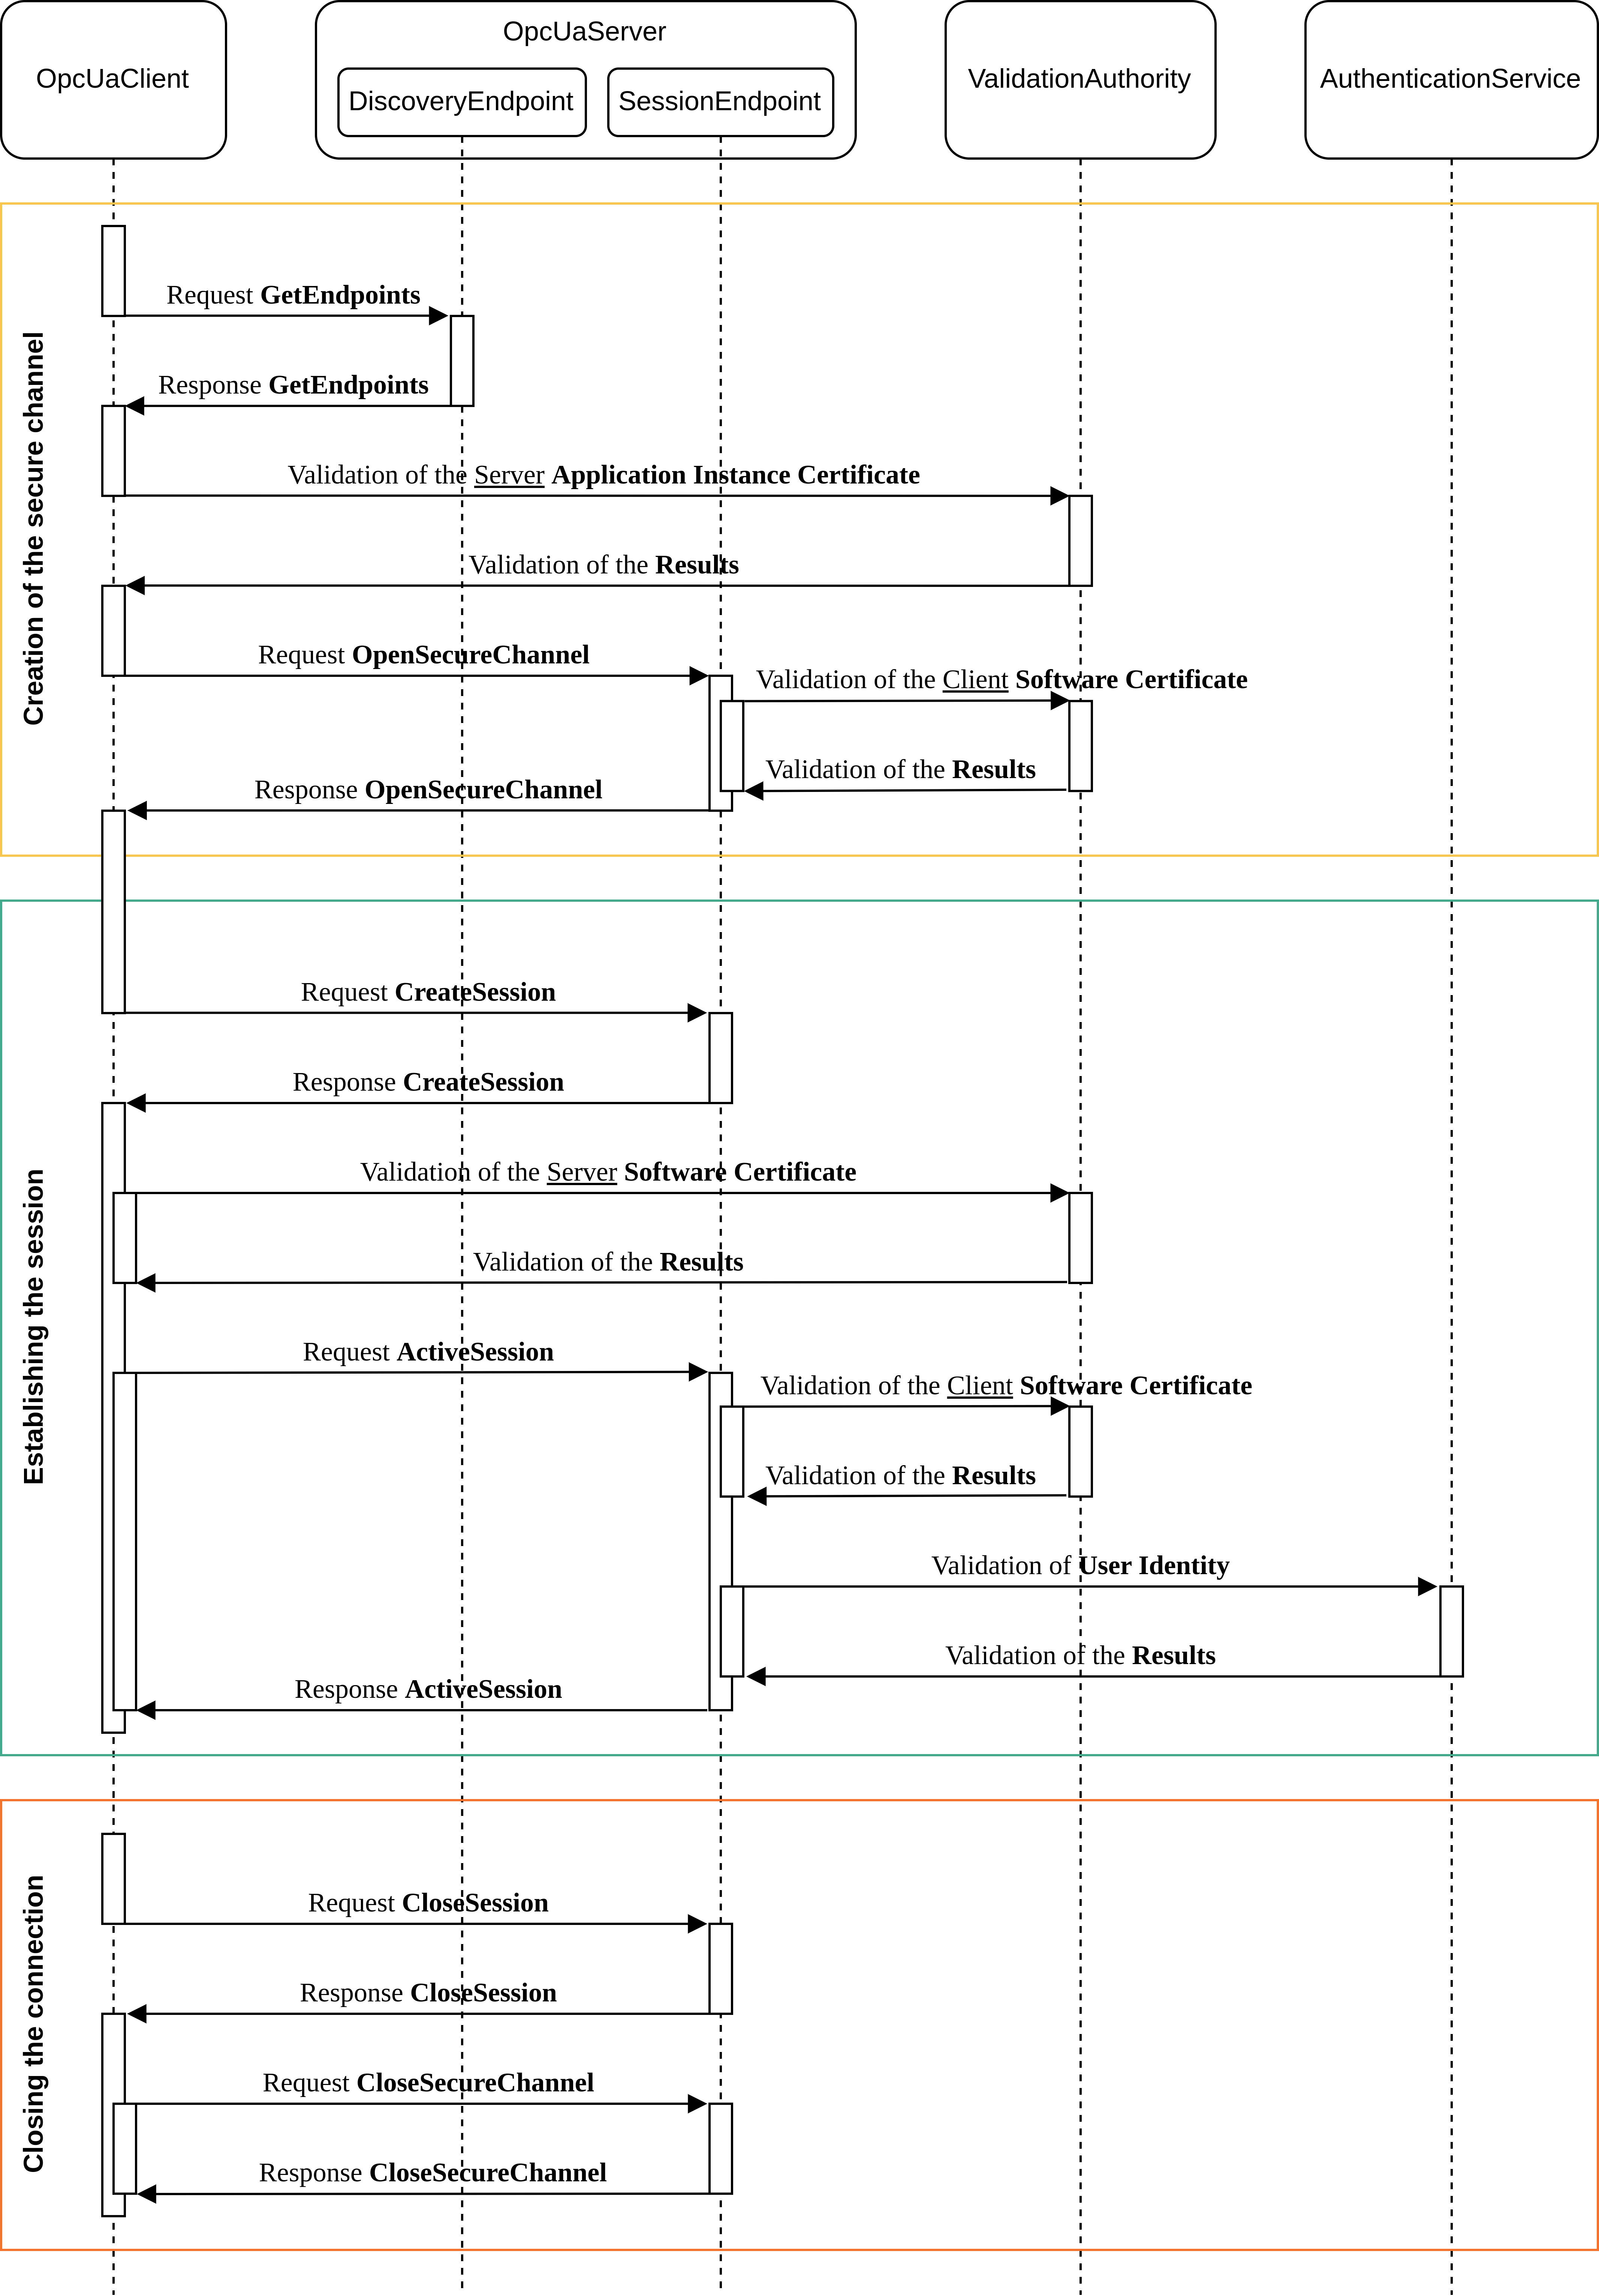
\includegraphics[width=\columnwidth]{high_quality/Fig1.png}
\caption{OPC UA connection creation and closure process}\label{fig1}
\end{figure}

Despite having a robust security system in place, OPC UA is vulnerable to different types of threats, particularly from the transport protocols with which it communicates. It is therefore critical to incorporate additional security protocols in networks to counteract such threats and make the system resilient against attacks.

The IEC 62443 standard establishes that in cases where the communication protocol has limitations that prevent reaching the Target Security Level (SL-T), compensatory countermeasures must be adopted. The components of an IACS do not provide the capabilities required to meet a given security level. In such scenarios, the use of compensating security measures, technical or procedural, can help to facilitate the needed capability. The combination of multiple techniques found within a security solution is designed to fulfill such a role \cite{iec62443-3-3}.
A widely used countermeasure is the use of VPN tunnels, often implemented through bump-in-the-wire firewalls, as presented in the works \cite{ghanen2022}, \cite{hohmann2021} and \cite{pudelko2020}. 

A systematic review of 238 studies by \cite{daSilva2023} presents an overall summary of emerging trends, unresolved questions, and challenges in the field of OPC UA. The review particularly highlights that there have been few publications considering the security aspects of OPC UA in the recent past, indicating that there is still not enough exploration in this aspect. Even though, based on its architecture that supports strong security services such as user authentication, information encryption, and fine-grained access control, the protocol faces issues that require further academic analysis. This could be due to a large number of guidelines adopted by the OPC Foundation for the safe use of OPC UA \cite{opcua2025}, which could reduce the urgency felt by researchers to further explore this aspect.

\subsection{Cyberattacks} \label{sec:cyberattacks}

Cyberattacks on IACS are malicious actions that are aimed at disrupting the integrity, confidentiality, or availability of operational assets \cite{turcato2020}. The convergence that has been achieved between IT/OT has enlarged the attack surface within these environments and has made vital infrastructure increasingly vulnerable to such threats. Cyber intrusions compromise weakly configured network configurations, software applications, or system settings, using them to disrupt physical operations, steal sensitive information, or create operational disruptions.

Attacks are essentially passive or active. Passive attacks are those that include eavesdropping on network communications without direct interference and mainly breach data confidentiality. The classic example is that of packet sniffing, where an attacker intercepts data packets and examines their contents and extracts intelligence for follow-up attacks. Active attacks, on the other hand, include altering the data stream or the state of the system. They may consist of altering legitimate messages, injecting malicious information, or causing service disruptions, and thus directly breaching the integrity and availability of the system.

Some active threats within industrial networks are Man-in-the-Middle (MITM) attacks, where an attacker secretly intercepts and may alter communications between two entities, and Denial-of-Service (DoS) attacks, which are designed to render a machine or network resource inoperable by inundating it with an intolerable number of requests or corrupted packets. MITM and DoS attacks are among the most common threats within industrial environments \cite{cekerevac2017}. Given their prevalence, this study focuses on sniffing, MITM, and DoS attack scenarios within an OPC UA network.

\section{Methodology}\label{sec:methodology}

\subsection{Experimental Testbed}

%The methodology applied involved the construction of an experimental testbench that mimics real-world industrial communication network environments where the OPC UA protocol is widely employed.
The methodology involved building an experimental testbed that mimics a real-world industrial network. This structure served as the experimental setup for a series of intrusion tests. Through the dynamic stimulation of various cyberattack strategies, the aim was to investigate vulnerabilities within two different domains, namely the application layer, which is concerned with the implementation and use of the OPC UA protocol, and the infrastructure layer, which is concerned with exploiting vulnerabilities within the underlying network configuration and host systems.

The testbench developed for this study included a variety of hardware components as well as software modules. The main components of the hardware are described in \autoref{tab:hardware}, while the software programs that were implemented to simulate operations and launch attacks are listed in \autoref{tab:software}. The schematic of the bench is presented in \autoref{fig:bench}.

\begin{table*}[ht]
\caption{List of hardware employed in the testbed}\label{tab:hardware}
\begin{tabular*}{\textwidth}{@{\extracolsep{\fill}}l p{0.18\textwidth} p{0.33\textwidth} p{0.35\textwidth}}
\toprule
Item & Equipment & Description & Function \\
\midrule
1 & DF63 NG & Nova Smar controller linking H1/HSE networks and native OPC UA. & Serves as the target industrial OPC UA device. \\
2 & Raspberry Pi 4 & Single-board computer for robust processing. & Hosts OPC UA client instances for testing. \\
3 & Ethernet Switch & TP-Link switch for centralizing network connections. & Interconnects all devices on the local test network. \\
4 & Attacker Machine & Configured computer running network attack/scan tools. & Originates simulated network attacks and scans. \\
\bottomrule
\end{tabular*}
% \footnotetext[1]{Utilized as an OPC UA client/server host.}
% \footnotetext[2]{Managed switch enabling traffic mirroring/manipulation.}
\end{table*}

\begin{table*}[ht]
\caption{List of software employed in the testbed} \label{tab:software}
\begin{tabular*}{\textwidth}{@{\extracolsep{\fill}}l p{0.18\textwidth} p{0.33\textwidth} p{0.35\textwidth}}
\toprule
Item & Software & Description & Function \\
\midrule
1 & Smar OPC UA Server & Proprietary Nova Smar server for O-PAS industrial systems. & Provides target secure OPC UA communication endpoint. \\
2 & opcua-asyncio & Open-source Python library for async OPC UA implementation. & SDK for building custom OPC UA clients/servers. \\
3 & OPC UA Exploit Framework & Open-source toolkit (Claroty) for OPC UA vulnerability research. & Facilitates OPC UA security testing \& exploit development. \\
4 & Ettercap & Network tool primarily used for MITM attacks. & Executes the attacks; intercepts and filters network traffic. \\
5 & Hping3 & Command-line TCP/IP packet assembler and analyzer tool. & Used for network scanning, packet crafting, and DoS tests. \\
6 & Wireshark & Open-source network packet capture and analysis software. & Captures and analyzes detailed network traffic for inspection. \\
7 & Nmap & Open-source tool for network discovery \& security auditing. & Scans networks to identify hosts, services, and open ports. \\
\bottomrule
\end{tabular*}
\end{table*}

\begin{figure}[htbp!]
\centering
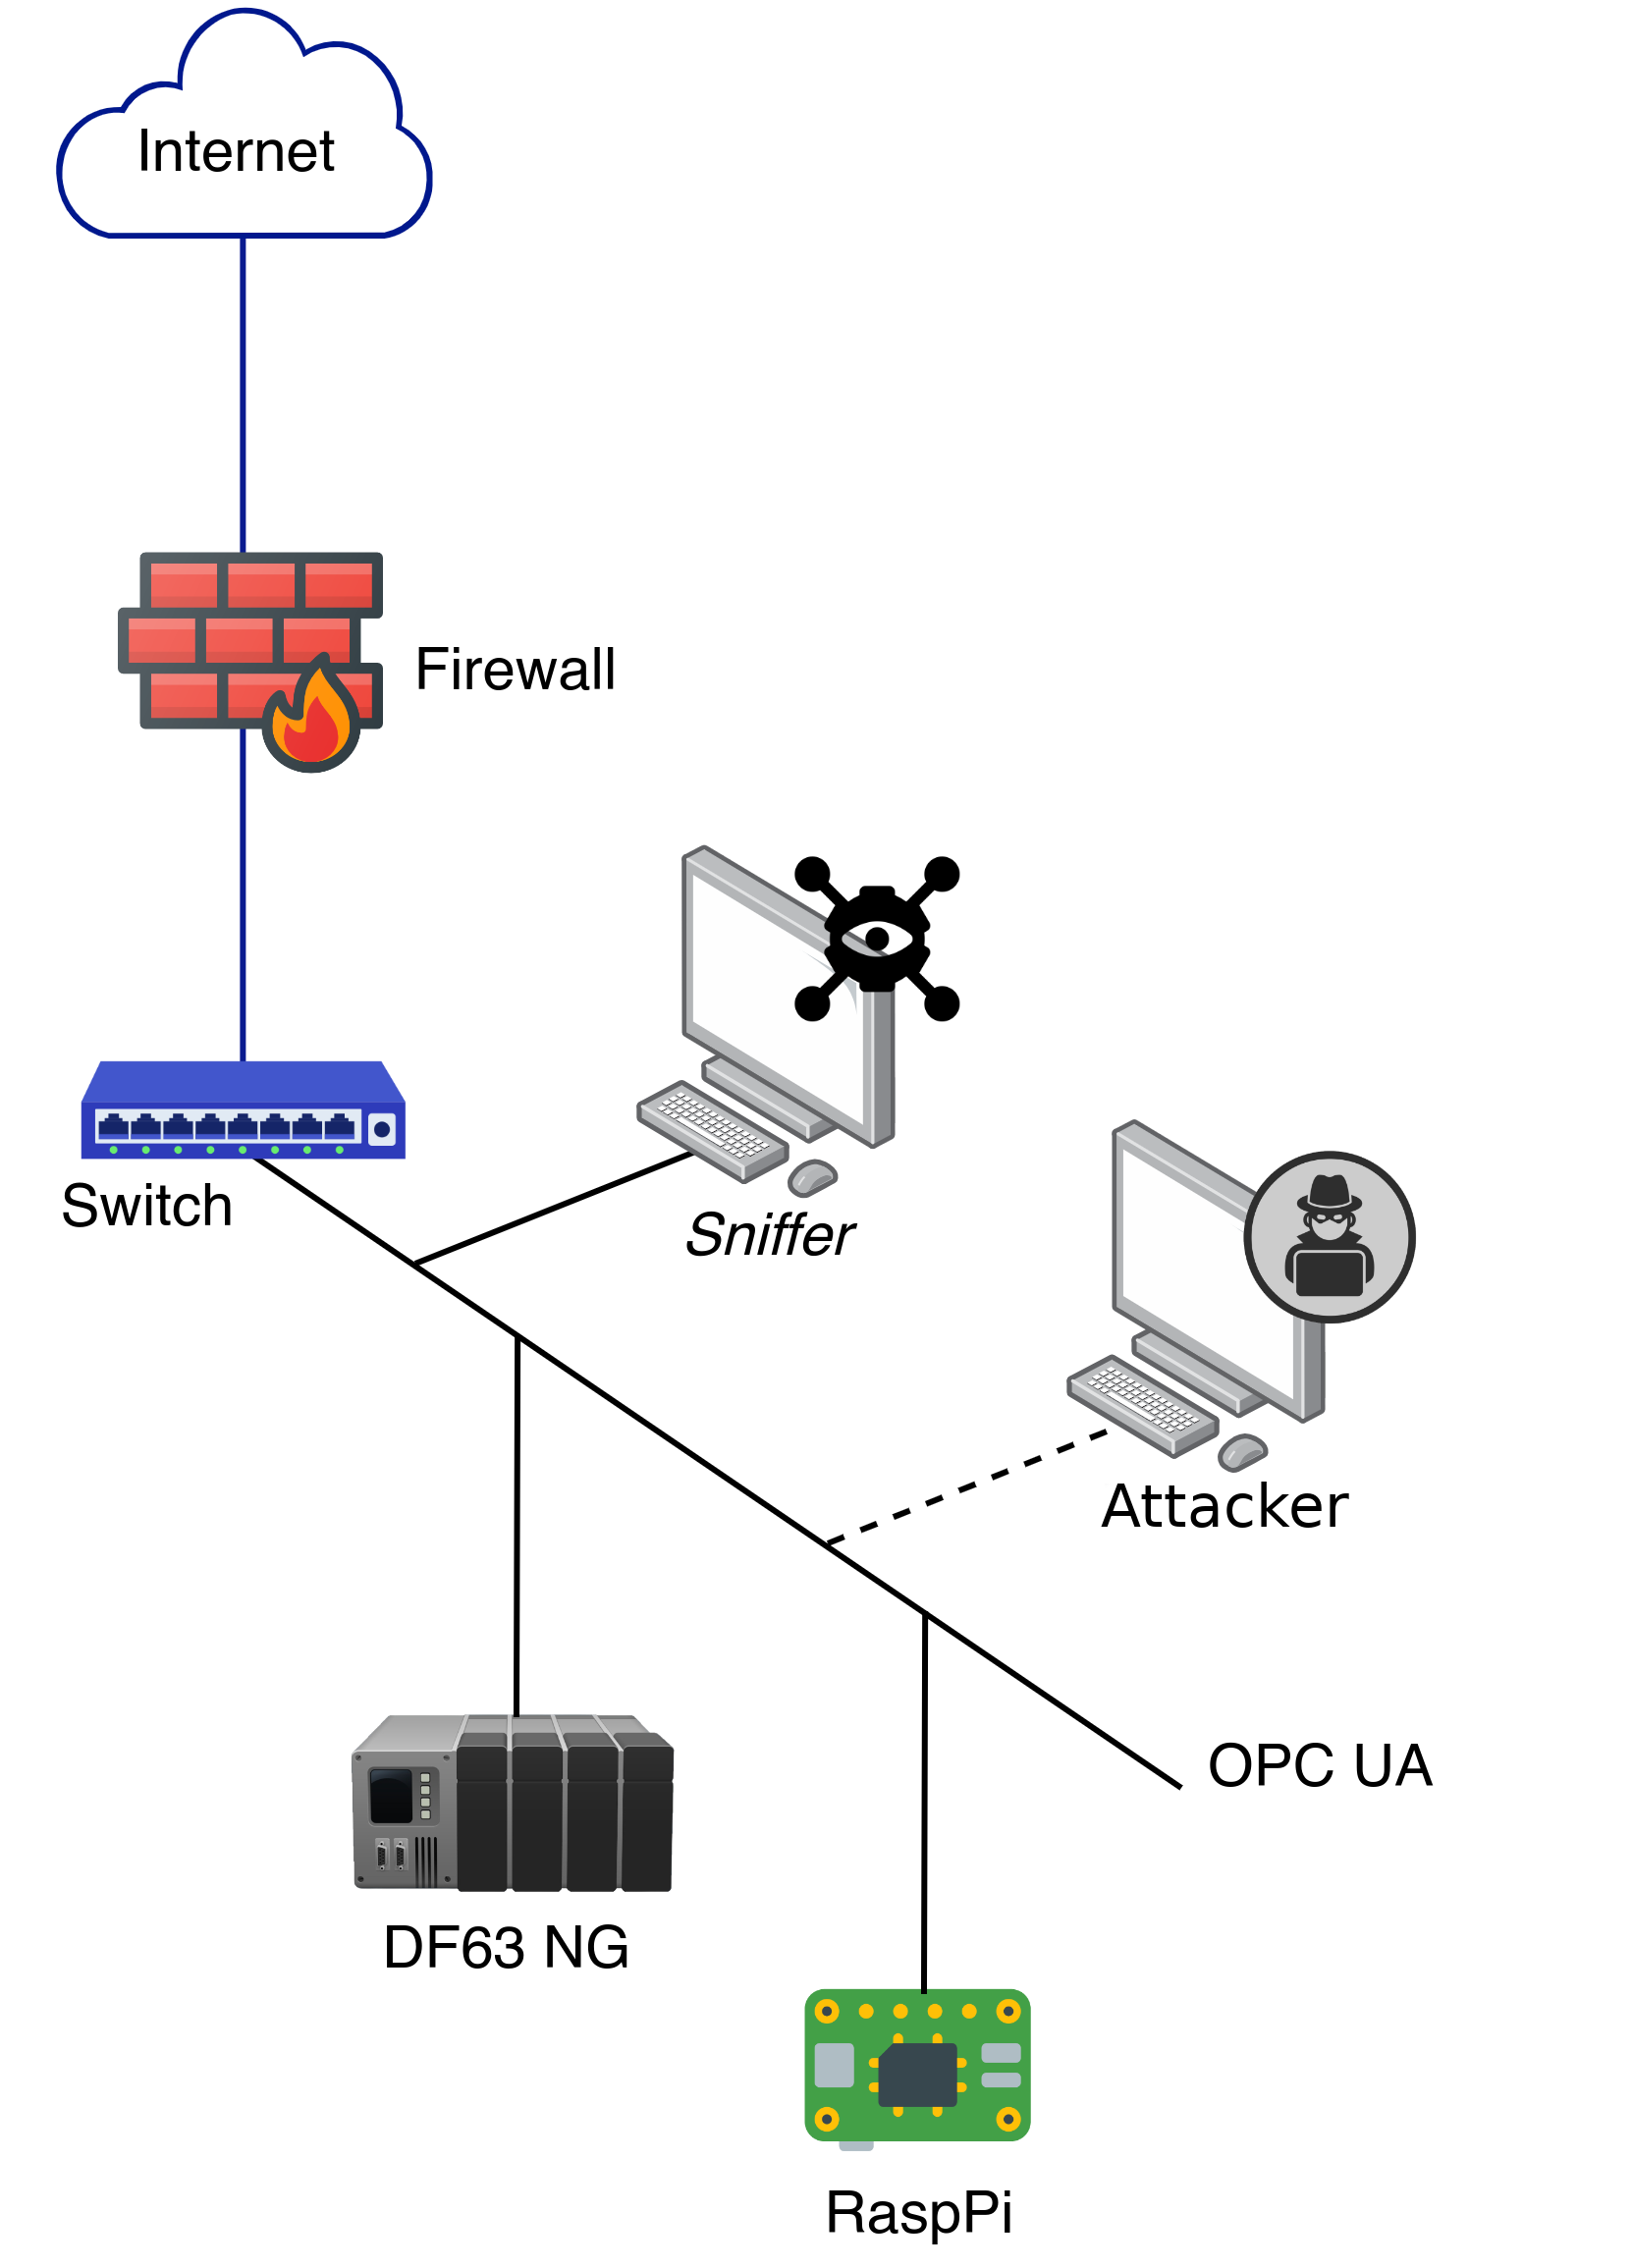
\includegraphics[width=0.35\textwidth]{high_quality/Fig2.png}
\caption{General schematic of the experimental testbench for cybersecurity testing}\label{fig:bench}
\end{figure}

\subsection{Investigated Cyberattack Scenarios}

Following the setup and working state of the OPC UA network testbench, a range of cyberattacks was launched. 

Initially, packet sniffing was performed. In this case, the attacker used Ettercap as the network interface sniffer on a managed switch, sniffing the live communications. The switch was configured to replicate the traffic shared between the OPC UA client and the server, sending copies of packets directly to the attacker to be captured. %At the same time, Wireshark was used to enable a more detailed analysis, providing the capability for a broad investigation of the captured data packets.

The second scenario involved MITM attacks. The first step was the network scan with the help of Ettercap to look for active hosts on the network. Next, more sophisticated approaches were used to achieve the MITM, such as ARP spoofing, in which devices are tricked into redirecting traffic to the attacker instead of the intended destination by corrupting their ARP tables, and port stealing, which involved the use of malicious ARP packets that actually hijack the target's switch port, sending packets intended for the victim to the attacker. In both packet sniffing and MITM attack environments, the use of Wireshark was instrumental, specifically filtering OPC UA protocol packets to compromised communication analysis.

The third scenario deals with DoS attacks. These types of attacks are not defined by their subtlety; instead, they are designed to overwhelm the system. The attacker can use untrusted clients or flood the server with a barrage of target messages, crippling the service, or even causing it to stop completely.
%The DoS flavors tested included: (1) SYN flooding, relentlessly hammering the server with connection requests; (2) ACK/ERR flooding, designed to force excessive error handling or acknowledgement responses from the server; (3) deliberately malformed message injection; (4) CLO flooding, inundating the server with channel closing requests; (5) repetitive bombardment with FindServers and GetEndpoints messages; and (6) combined SYN and OPN attacks, focusing on the computationally heavier certificate validation process, 
% which \cite{neu2019} highlights as particularly critical when the certificate authority resides on a separate system. 

The tools utilized in these DoS activities included the OPC UA Exploit Framework, Hping3 for creating and sending customized packets -- specifically for SYN flood attacks involving the specification of packet type, destination port or IP address, and often a spoofed source IP address --, and Nmap, which was used in this case mainly for its stealth SYN scan feature to anonymously determine active IP addresses and ports before launching an attack.

In addition to analyzing basic attacks, the study also explored more advanced areas, leveraging existing vulnerabilities also covered by the OPC UA Exploit Framework \cite{claroty2023}. The scenarios in question consisted of attacks targeting specific implementation flaws related to certificate processing (Infinite Certificate Chain Loop), memory management (Null Pointer Dereference), resource exhaustion from excessive secure channel (Multiple Secure Channel Opening), and navigation requests (Path Translation Attack). A detailed evaluation of the effectiveness and impact of all tested scenarios is provided in the \nameref{sec:results}.

\subsection{Data Acquisition and Processing}

The data collection phase used Wireshark to capture network traffic in different simulated cyberattack scenarios during client-server communication. In each case, a 60-second capture session was performed to ensure consistency, and then the captures were saved as \textbf{.pcapng} files. The file naming convention was systematic, indicating the OPC UA security mode (\textit{None}, \textit{Sign}, \textit{Sign\&Encrypt}), the attack type, and a sequence capture number.

Together with the inspection of communication packets, server performance metrics, specifically CPU and RAM usage, were evaluated by running custom scripts triggered by the Sniffer process. This allowed for an integrated analysis of network events along with their computational implications. Each experimental condition, defined in terms of attack type and security setting, was repeated multiple times in a controlled environment with consistent network settings to improve the validity of the findings.

The raw data, which were large amounts of packets and performance data, were processed using \textbf{uanalyser}, a custom Python tool developed for the scope of this investigation. This tool translates complex data into understandable outputs, which were graphical representations of four key metrics: network throughput (kbps), server CPU and RAM usage (in percentage), OPC UA packet rate (packets per second) and normalized Round-Trip Time (RTT). The \textbf{uanalyser} source code is publicly available on GitHub. \footnote{\label{github_note}Available at: \url{https://github.com/JonathanTSilva/opcua-analyser}. Accessed: 14 April 2025}
%The tool's functionality was supported through the use of several Python libraries, such as Scapy for processing packets, and Matplotlib, NumPy, and Pandas for visualization, numerical calculations, and data handling, respectively.

\section{Results}\label{sec:results}

The testbed was configured according to the \autoref{sec:methodology} to execute the defined attack scenarios.  A detailed result is described in \autoref{tab:combined-results}. 
%which clarifies network traffic behavior and system performance along with providing essential classification of results that arose from every attack.

They were classified according to how effectively the attack fulfilled its objectives, particularly with respect to the core principles of secure communication. The results are generally referred to as follows:

\begin{itemize}
    \item Success: indicates that the attack was carried out without encountering sufficient countermeasures, successfully accomplishing its task to compromise an essential element of security, defined by the CIA triad or the AAA framework;
    \item Failure: the attack failed to achieve its intended goal or was effectively mitigated.
\end{itemize}

\begin{table*}[ht]
    \centering
    \caption{Attack results and network characteristics per scenario}
    \label{tab:combined-results}
    \begin{tabular*}{\textwidth}{@{\extracolsep\fill}l l l c c c c r}
        \toprule
        Scenario & Attack Type & Security Mode & AT\footnotemark[1] & APL\footnotemark[2] & APPS\footnotemark[3] & ACPU\footnotemark[4] & Result \\
        \midrule
        C1 & \multirow{3}{*}{\parbox{2.5cm}{DoS via infinite loop in certificate chain}} & None & 130 & 127 & 128.4 & 7.31 & Failure \\
        C2 & & Sign & 175 & 153 & 142.9 & 8.91 & Failure \\
        C3 & & Sign\&Encrypt & 179 & 162 & 138.3 & 9.01 & Failure \\
        \midrule
        C4 & \multirow{3}{*}{\parbox{2.5cm}{DoS via null pointer dereferencing}} & None & 1166 & 965 & 151.1 & 17.16 & Success \\
        C5 & & Sign & 6824 & 972 & 877.9 & 10.64 & Success \\
        C6 & & Sign\&Encrypt & 6894 & 973 & 885.9 & 10.78 & Success \\
        \midrule
        C7 & \multirow{3}{*}{\parbox{2.5cm}{DoS via TCP/IP flooding}} & None & 18000 & 60 & 38438.9 & 14.68 & Success \\
        C8 & & Sign & 12000 & 60 & 26788.9 & 13.23 & Success \\
        C9 & & Sign\&Encrypt & 15000 & 60 & 31278.5 & 14.81 & Success \\
        \midrule
        C10 & \multirow{3}{*}{\parbox{2.5cm}{DoS via multiple secure channels}} & None & 462 & 171 & 337.3 & 9.86 & Failure \\
        C11 & & Sign & 501 & 180 & 348.0 & 11.27 & Failure \\
        C12 & & Sign\&Encrypt & 491 & 184 & 334.1 & 11.36 & Failure \\
        \midrule
        C13 & \multirow{3}{*}{\parbox{2.5cm}{DoS via navigation path translation}} & None & 196 & 173 & 141.4 & 7.52 & Failure \\
        C14 & & Sign & 235 & 195 & 151.3 & 9.03 & Failure \\
        C15 & & Sign\&Encrypt & 247 & 203 & 152.6 & 9.09 & Failure \\
        \midrule
        C16 & \multirow{3}{*}{\parbox{2.5cm}{MITM via ARP table spoofing}} & None & 105 & 125 & 105.3 & 6.80 & Success \\
        C17 & & Sign & 146 & 148 & 123.4 & 7.84 & Success \\
        C18 & & Sign\&Encrypt & 137 & 159 & 107.9 & 7.96 & Failure \\
        \midrule
        C19 & \multirow{3}{*}{\parbox{2.5cm}{MITM via port stealing}} & None & 3410 & 43 & 10012.0 & 7.36 & Success \\
        C20 & & Sign & 3433 & 43 & 9896.4 & 7.97 & Success \\
        C21 & & Sign\&Encrypt & 3432 & 44 & 9854.8 & 7.97 & Failure \\
        \midrule
        C22 & \multirow{3}{*}{\parbox{2.5cm}{Packet sniffing}} & None & 168 & 127 & 166.1 & N/A & Success \\
        C23 & & Sign & 223 & 154 & 182.4 & N/A & Success \\
        C24 & & Sign\&Encrypt & 219 & 162 & 169.7 & N/A & Failure \\
        \midrule
        C25 & \multirow{3}{*}{\parbox{2.5cm}{Normal communication}} & None & 95 & 121 & 98.5 & 7.01 & N/A \\
        C26 & & Sign & 253 & 142 & 222.7 & 7.95 & N/A \\
        C27 & & Sign\&Encrypt & 234 & 147 & 199.8 & 8.25 & N/A \\
        \bottomrule
    \end{tabular*}
    \footnotetext[1]{AT (Average Throughput): Average data rate measured in kilobits per second (kbit/s).}
    \footnotetext[2]{APL (Average Packet Length): Average size of network packets measured in bytes.}
    \footnotetext[3]{APPS (Average Packets per Second): Average number of packets transmitted per second (packets/s).}
    \footnotetext[4]{ACPU: Average CPU usage of the OPC UA server host, expressed as a percentage (\%).}
\end{table*}

It should be noted that the AT, APL, APPS, and ACPU metrics were collected over a 60-second window, capturing all network traffic rather than isolating attack-specific packets. Although thorough, this broad approach can obscure the impact of short-lived attacks, potentially understating their severity. For example, in TCP/IP flooding scenarios (C7–C9), where APPS hit 38,438.9 packets/s, averaged values might mask brief spikes that crippled the system.

This methodological nuance emphasizes the need for real-time monitoring in industrial settings, where even fleeting disruptions can trigger major operational failures. The data provides a solid basis for analyzing attack impacts, but pinpointing transient vulnerabilities demands a more granular survey.

The contrast between attack types reveals OPC UA's uneven resilience. Scenarios C4–C6 (null pointer dereferencing) stand out, with AT soaring to 6,894 kbit/s in C6 (Sign\&Encrypt) and CPU usage peaking at 17.16\% in C4 (\textit{None}). These attacks exploit software flaws, bypassing security and straining resources.

In contrast, normal communication (C25–C27) showed stable metrics—AT between 95 and 253 kbit/s, ACPU below 8.25\%—highlighting a baseline that collapses under targeted exploits. This gap urges developers to patch vulnerabilities and optimize resources to prevent service disruptions in critical systems.

MITM attacks, especially port stealing (C19–C21), expose a critical weakness. With APPS around 10,000 packets/s and AT exceeding 3,400 kbit/s, these attacks succeeded across security modes with minimal CPU load (around 7.97\%). Even with Sign\&Encrypt, cryptographic defenses couldn’t stop network-layer manipulations.

% This vulnerability underscores the need for layered protections, such as Virtual Local Area Network (VLAN) segmentation or intrusion detection, to shield OPC UA networks from stealthy traffic-hijacking threats. Strengthening these defenses is vital for robust industrial operations.

The subsequent subsections offer a short overview of the outcomes for each attack scenario, accompanied by selected examples of the graphs employed in this study. To maintain brevity, not all graphs are included here; however, with access to the capture files and the custom software developed for this research, all visualizations can be easily reproduced. This approach ensures transparency while focusing on key illustrative findings \footnoteref{github_note}.

\subsection{Packet Sniffing}

Even with the secure channel feature enabled, the use of less secure security modes, namely \textit{None} and \textit{Sign} (C22 and C24), allowed an attacker to intercept packets with sensitive data such as IP addresses, MAC addresses, and commands sent to the server.

However, configuring communication with the `Sign\&Encrypt' security mode, utilizing algorithms such as Basic256Sha256, effectively encrypted transmitted data, rendering it inaccessible even after interception. This clearly demonstrates the efficacy of robust encryption in safeguarding message integrity and confidentiality.

\subsection{MITM}

After a successful phase of packet sniffing, an attacker gains important information about the device, including the OPC UA server address and \texttt{EndpointURI}, thus setting in motion the prerequisites for MITM. Through the ARP spoofing technique (C16-C18), the attacker was able to intercept and reroute data traffic, inserted between the client and the server. During such an engagement, it became possible to intercept and manipulate packets in transit, including \texttt{OpenSecureChannelRequest} and \texttt{CreateSessionRequest} messages involved in session setup. In a different approach (C19-C21), an MITM attack enabled by port stealing resulted in a dramatic throughput increase due to a large number of ARP packets flooding the server table. Although efficient, this method does not immediately divert all communication through the attacker but uses the hijacked port as a pass-through.

As illustrated in \autoref{fig:0-mitm-wireshark} and \autoref{fig:1-mitm-wireshark}, the capture of the packet reveals the communication dynamics between the OPC UA server and client, with an attacker cleverly placed as an intermediary. By examining the traffic, it is plain as day that the usual data flow is rerouted through the attacker, marked by the MAC address \textbf{00:09:5B:A0:5F:F0}. This deviation, plain and simple, highlights the attacker's ability to intercept and manipulate the data stream, revealing a critical vulnerability in the defenses of the network.

\begin{figure*}[htbp!]
\centering
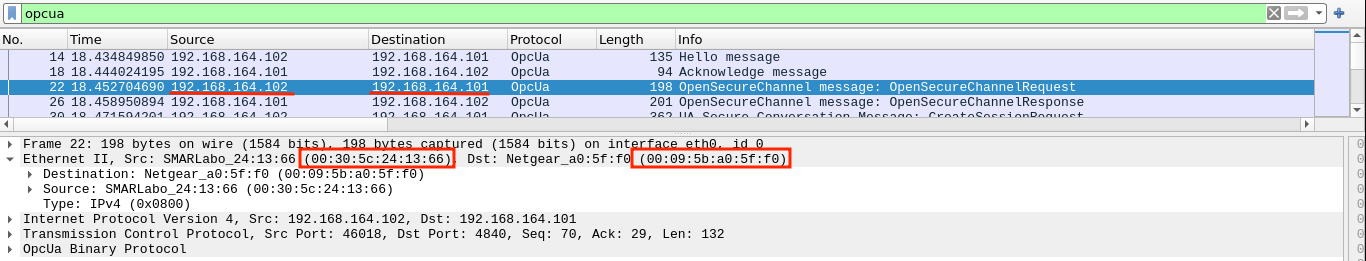
\includegraphics[width=1\textwidth]{high_quality/Fig3.png}
\caption{Interception of OpenSecureChannelRequest packets in the MITM attack with security mode `None'}\label{fig:0-mitm-wireshark}
\end{figure*}

\begin{figure*}[htbp!]
\centering
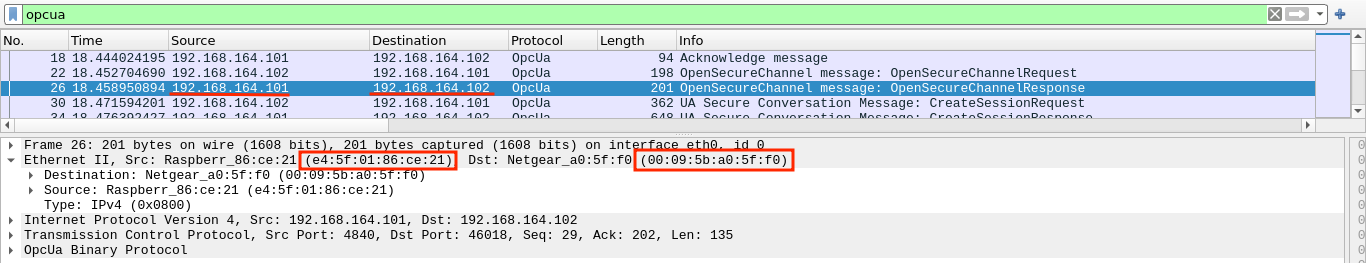
\includegraphics[width=1\textwidth]{high_quality/Fig4.png}
\caption{Interception of OpenSecureChannelResponse packets in the MITM attack with security mode `None'}\label{fig:1-mitm-wireshark}
\end{figure*}

\subsection{DoS}

Every DoS attack unleashed, without exception, triggered a jaw-dropping average increase of 420\% in the processing demand of the OPC UA server host, as vividly illustrated in \autoref{fig:dos1}. However, it should be noted that no other processes were running on the host during these controlled tests. In a real-world setting, this spike could spell disaster, potentially leading to a complete collapse of communication in all scenarios.

\begin{figure}[htbp!]
\centering
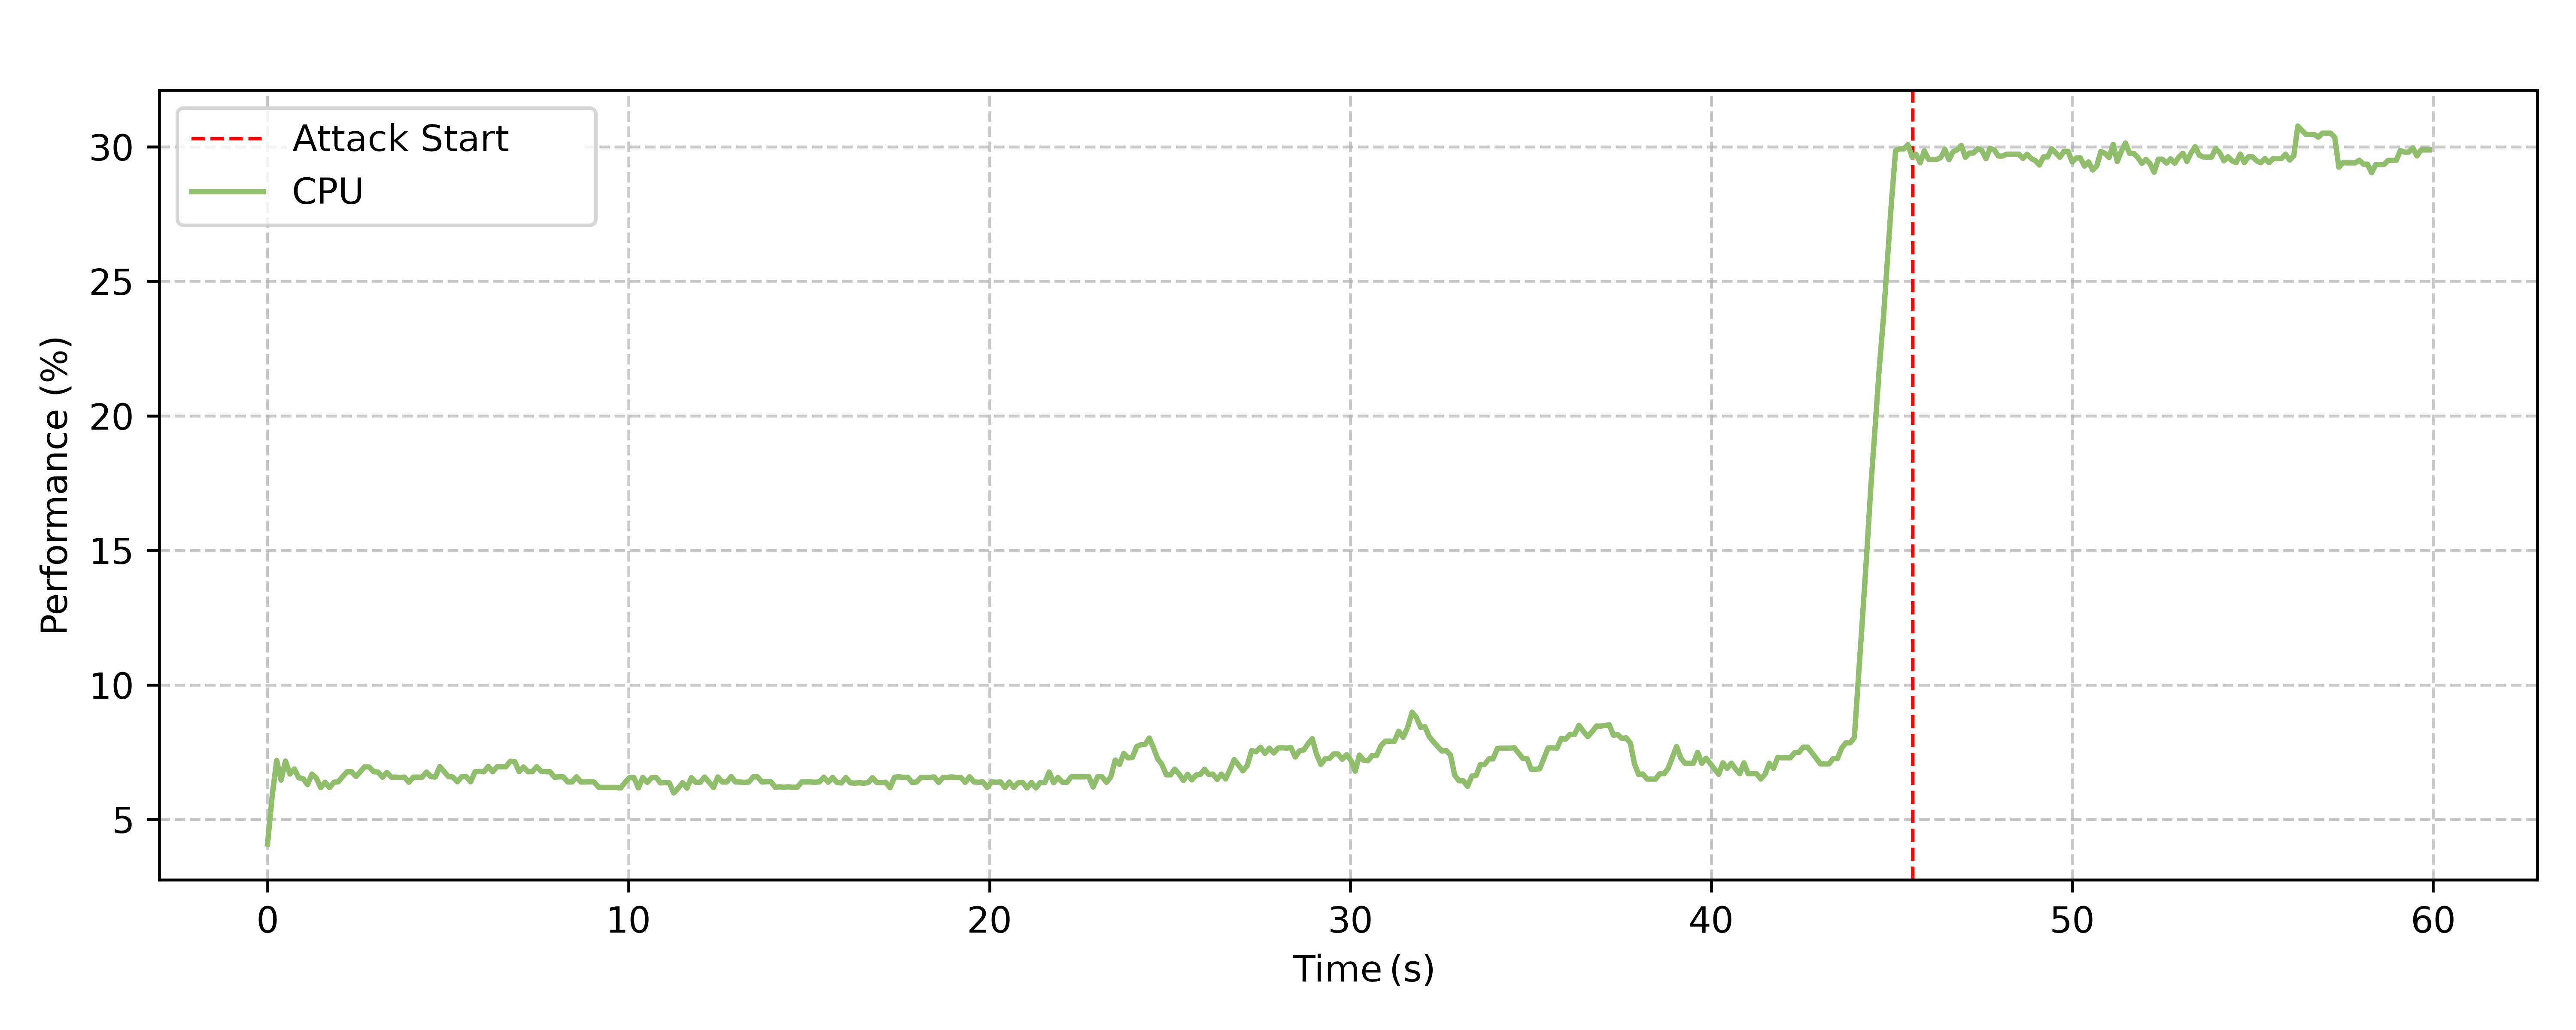
\includegraphics[width=\columnwidth]{high_quality/Fig5.png}
\caption{Average variation in the OPC UA server host processing during the TCP/IP flood attack in `Sign' mode}\label{fig:dos1}
\end{figure}

The following discussion summarizes the findings from five different DoS attack methods, each designed to test the resilience of an industrial OPC UA network under extreme loads. 

\begin{itemize}
    \item TCP/IP Flood: the network showed high vulnerability to TCP/IP flood attacks, with a spike in CPU usage and a significant increase in throughput, leading to degraded performance. Although not directly targeting the OPC UA protocol, the attack disrupted the underlying transport layer, highlighting the need for robust network infrastructure protection;
    \item Infinite Certificate Chain Loop: the OPC UA server proved resilient, maintaining stable client-server communication despite increased RTT for the attacker. This robustness, especially under secure configurations, underscores the protocol's strength against certain DoS attacks;
    \item Null Pointer Dereference: this attack caused a complete DoS across all tested scenarios, exploiting a critical server vulnerability. A sharp rise in CPU usage and throughput, followed by a communication collapse, revealed the urgent need for pointer validation to prevent such failures;
    \item Multiple Secure Channel Opening: simultaneous connection requests overwhelmed the server, spiking throughput (\autoref{fig:tput-ex2}), response time, and CPU usage. This overload exposed a critical weakness in handling excessive secure channel demands, leading to service disruptions;
    \item Path Translation Attack: exploiting the \texttt{TranslateBrowsePathsToNodeIds} function with long paths caused partial vulnerability through recursive overload. While some protection mitigated stack exhaustion, increased response times indicated performance degradation under attack.
\end{itemize}


\begin{figure}[htbp!]
\centering
\includegraphics[width=\columnwidth]{high_quality/Fig6.png}
\caption{OPC UA network throughput and packet rate during a DoS attack via Multiple Secure Channel Openings using the `None' mode}\label{fig:tput-ex2}
\end{figure}

\section{Key Improvements and Mitigations}

Industrial OPC UA network protection requires a comprehensive, multi-level method and conceives security as a dynamic process instead of a pre-established setting. Cyber resilience is achieved in a genuine manner by the precise improvement of applications, the implementation of robust protocol settings, and the use of Defense-in-Depth or Zero Trust network design. These fundamental ingredients align themselves with established guidelines such as IEC 62443 and emphasize the use of proactive management and real-time monitoring across the entire system lifecycle.

Strengthening the OPC UA implementation itself is the first line of defense to mitigate potential vulnerabilities. The success of the Null Pointer Dereference attack highlights the critical need to keep all IACS components updated with the latest security patches. Beyond maintenance, enforcing correct security policies is crucial. %The `Sign\&Encrypt` security mode was the only effective countermeasure against sniffing and Man-in-the-Middle attacks and should be mandated for all critical communications.

Strong authentication and access control must also be enforced. Anonymous access to critical resources should be strictly prohibited. Implementing robust authentication, such as Multi-Factor Authentication (MFA), combined with the principle of least privilege through Role-Based Access Control (RBAC) is essential to limit an attacker's potential impact.

Additionally, a rigorous certificate management lifecycle is necessary to mitigate risks like the certificate chain loop attack. Using a trusted Certificate Authority (CA) and securely storing private keys is crucial. Finally, enabling and actively monitoring detailed audit logs is vital for the early detection of anomalous activity, such as the flood of connection requests seen in the multiple secure channel attack.

However, securing the protocol is insufficient without hardening the underlying network. To counter threats at the network level, MITM attacks can be mitigated by configuring switch features like port security and using static ARP entries for critical devices. The network architecture should also incorporate segmentation through Virtual Local Area Networks (VLANs) to contain threats and limit an attacker's lateral movement.

For active defense, the deployment of Intrusion Detection and Prevention Systems (IDS/IPS) provides essential real-time monitoring. These systems can detect the anomalous traffic patterns characteristic of the attacks performed in this study. To unify these defenses, a Security Information and Event Management (SIEM) system should be implemented. A SIEM aggregates and correlates logs from all sources—switches, firewalls, and OPC UA servers—to enable the early detection of complex, multi-stage attacks. A monitoring system could also be supplemented by AI. Successful attacks consistently created spikes in the kind of metrics used in this study: throughput, packet rate, and host performance. An AI model trained to identify such peaks as malicious activity would counter threats proactively before they affect important industrial operations. % A monitoring framework could be further enhanced with AI, as successful attacks consistently produced dramatic spikes in metrics like throughput, packet rate, and host performance. An AI model trained to recognize these peaks as malicious behavior could proactively mitigate threats before they impact critical industrial operations.

\section{Conclusion}\label{sec13}

This investigation successfully identified and analyzed vulnerabilities within industrial OPC UA networks by employing an experimental testbed designed to simulate a range of cyberattack scenarios. The empirical data gathered enabled a rigorous assessment of the OPC UA protocol's security features and the resilience of associated network components when challenged by diverse threat vectors. The outcomes highlighted both the inherent strengths of the protocol and specific areas that could be susceptible to exploitation if not adequately configured and managed, thereby offering a nuanced view of its robustness in operational environments.

The research demonstrated that while OPC UA possesses foundational security mechanisms, certain attack vectors can significantly compromise system integrity. For example, DoS attacks, particularly those leveraging null pointer dereferencing or the overwhelming of servers through multiple secure channel requests, were found to be notably effective, capable of causing service outages or critical server strain. Conversely, the protocol exhibited commendable resilience against other threats, such as infinite loop attacks targeting certificate chains, maintaining service quality for legitimate communications under duress. A key finding emphasized the crucial role of appropriate security mode configurations, with `Sign\&Encrypt' proving essential in safeguarding data confidentiality and integrity against packet sniffing and MITM attacks.

%%===================================================%%
%% For presentation purpose, we have included        %%
%% \bigskip command. Please ignore this.             %%
%%===================================================%%
% \bigskip
% \begin{flushleft}%
% Editorial Policies for:

% \bigskip\noindent
% Springer journals and proceedings: \url{https://www.springer.com/gp/editorial-policies}

% \bigskip\noindent
% Nature Portfolio journals: \url{https://www.nature.com/nature-research/editorial-policies}

% \bigskip\noindent
% \textit{Scientific Reports}: \url{https://www.nature.com/srep/journal-policies/editorial-policies}

% \bigskip\noindent
% BMC journals: \url{https://www.biomedcentral.com/getpublished/editorial-policies}
% \end{flushleft}

%%===========================================================================================%%
%% If you are submitting to one of the Nature Portfolio journals, using the eJP submission   %%
%% system, please include the references within the manuscript file itself. You may do this  %%
%% by copying the reference list from your .bbl file, paste it into the main manuscript .tex %%
%% file, and delete the associated \verb+\bibliography+ commands.                            %%
%%===========================================================================================%%

\bibliography{sn-bibliography}% common bib file
%% if required, the content of .bbl file can be included here once bbl is generated
%%\input sn-article.bbl


\end{document}
